%% Preamble
\documentclass[usenames,dvipsnames,tikz]{article}

%% Dependencies
\usepackage{xeCJK}
\usepackage[T1]{fontenc}
\usepackage[utf8]{inputenc}
\usepackage{amsmath}
\usepackage{color}
\usepackage{xcolor}
\usepackage[b4paper,landscape,nohead,margin=2cm]{geometry}
\usepackage{tikz}
\usepackage{tikz-cd}
\usetikzlibrary{shapes,mindmap,shadows,backgrounds}
\usetikzlibrary{cd,matrix}

%% Settings
\definecolor{shallowyellow}{RGB}{245,245,204}
\def\anno#1#2#3{\node [anno,#3] at (#2) {\textbf{\large #1}}}
\def\annop#1#2{\node [anno,xshift=-5cm] at (#2) {\textbf{\large #1}}}
\makeatletter
\tikzset{
column sep/.code=\def\pgfmatrixcolumnsep{\pgf@matrix@xscale*(#1)},
row sep/.code =\def\pgfmatrixrowsep{\pgf@matrix@yscale*(#1)},
matrix xscale/.code=\pgfmathsetmacro\pgf@matrix@xscale{\pgf@matrix@xscale*(#1)},
matrix yscale/.code=\pgfmathsetmacro\pgf@matrix@yscale{\pgf@matrix@yscale*(#1)},
matrix scale/.style={/tikz/matrix xscale={#1},/tikz/matrix yscale={#1}}}
\def\pgf@matrix@xscale{1}
\def\pgf@matrix@yscale{1}
\makeatother

%% Stylish
\pagestyle{empty}
\pagecolor{shallowyellow}
\tikzstyle{root}+=[font=\Huge]
\tikzstyle{node}+=[concept color=teal]
\tikzstyle{cons}+=[concept color=purple]
\tikzstyle{chain}+=[concept color=darkgray]
\tikzstyle{anno}=[annotation,everynode,above,fill=black!50,text width=8cm,inner sep=4mm]
\tikzstyle{group}+=[mindmap,grow cyclic,concept color=darkgray,every node/.append style={everynode,concept}]
\tikzstyle{catethe}=[inner sep=12mm,row sep=2em,column sep=3em]
\tikzstyle{everynode}+=[text=white,scale=1.2,circular drop shadow]
\tikzstyle{level 1 concept}+=[level distance=5.2cm,font=\Large]
\tikzstyle{level 2 concept}+=[level distance=3.8cm,font=\large]
%\tikzstyle{level 3 concept}+=[level distance=2.3cm,font=\scriptsize,rotate=30]
%\tikzstyle{level 4 concept}+=[level distance=1.6cm,font=\tiny]

%% Document
\begin{document}
  \begin{tikzpicture}
    \path[group]
    node[root] (chain1) at (0,0) {$Chain_1$}
    child[node] {node (node1) {$Node_1$}}
    child[node] {node (node2) {$Node_2$}}
    child[cons] {node (pow) {$PoW$}};
    \path[group]
    node[root] (chain2) at (10,-7) {$Chain_2$}
    child[node] {node (node3) {$Node_3$}}
    child[node] {node (node4) {$Node_4$}}
    child[node] {node (node5) {$Node_5$}}
    child[cons] {node (pos) {$PoS$}};
    \path[group]
    node[root] (chain3) at (-12,-4) {$Chain_3$}
    child[cons,clockwise from=90] {node (poa) {$PoA$}};
    \path (node1) to [circle connection bar switch color = from (teal) to (darkgray)] (chain2);
    \path (node1) to [circle connection bar switch color = from (teal) to (darkgray)] (chain3);
    \path (node3) to [circle connection bar switch color = from (teal) to (darkgray)] (chain3);
    \path (chain1) to [circle connection bar switch color = from (darkgray) to (darkgray)] (chain2);
    \path (chain1) to [circle connection bar switch color = from (darkgray) to (darkgray)] (chain3);
    \annop{假设一个运行于 BCID2.0 下的拓扑网络中的所有节点呈现以下分布}{chain1.north};
  \end{tikzpicture}
  \newpage

  \begin{tikzpicture}
    \path[group,node,level 1/.append style={sibling angle=120}]
    node[root] (node) {$Node_1$}
    child[chain] {node {$Chain_1$} child[cons] {node {$PoW$}}}
    child[chain] {node {$Chain_2$} child[cons] {node {$PoS$}}}
    child[chain] {node {$Chain_3$} child[cons] {node {$PoA$}}};
    \annop{那么对于单个节点而言,比如 ${\mathrm{Node_1}}$ ,它的运行环境是这样的}{node.west};
  \end{tikzpicture}
  \newpage

  \begin{tikzpicture}
    \path
    node[scale=2,fill=black!15,rounded corners=4mm] (cate) {
    \begin{tikzcd}[catethe,matrix scale=1.4]
      Node_2 \ar[r, "f"] \ar[rd, orange, "g \circ f"] & Node_1 \ar[d, teal, "g"] \\
      PoX & Chain \ar[l, red] & Node_a \ar[l, teal] \\
      & Node_c \ar[u, teal] & Node_b \ar[lu, teal]
    \end{tikzcd}};
    \anno{对于一个局部共识 G1,当节点 $\mathrm{Node_2}$ 尝试通过连接 $\mathrm{Node_1}$ 加入到共识中时}{cate.north}{yshift=1cm};
  \end{tikzpicture}
  \qquad\qquad\qquad\qquad\qquad
  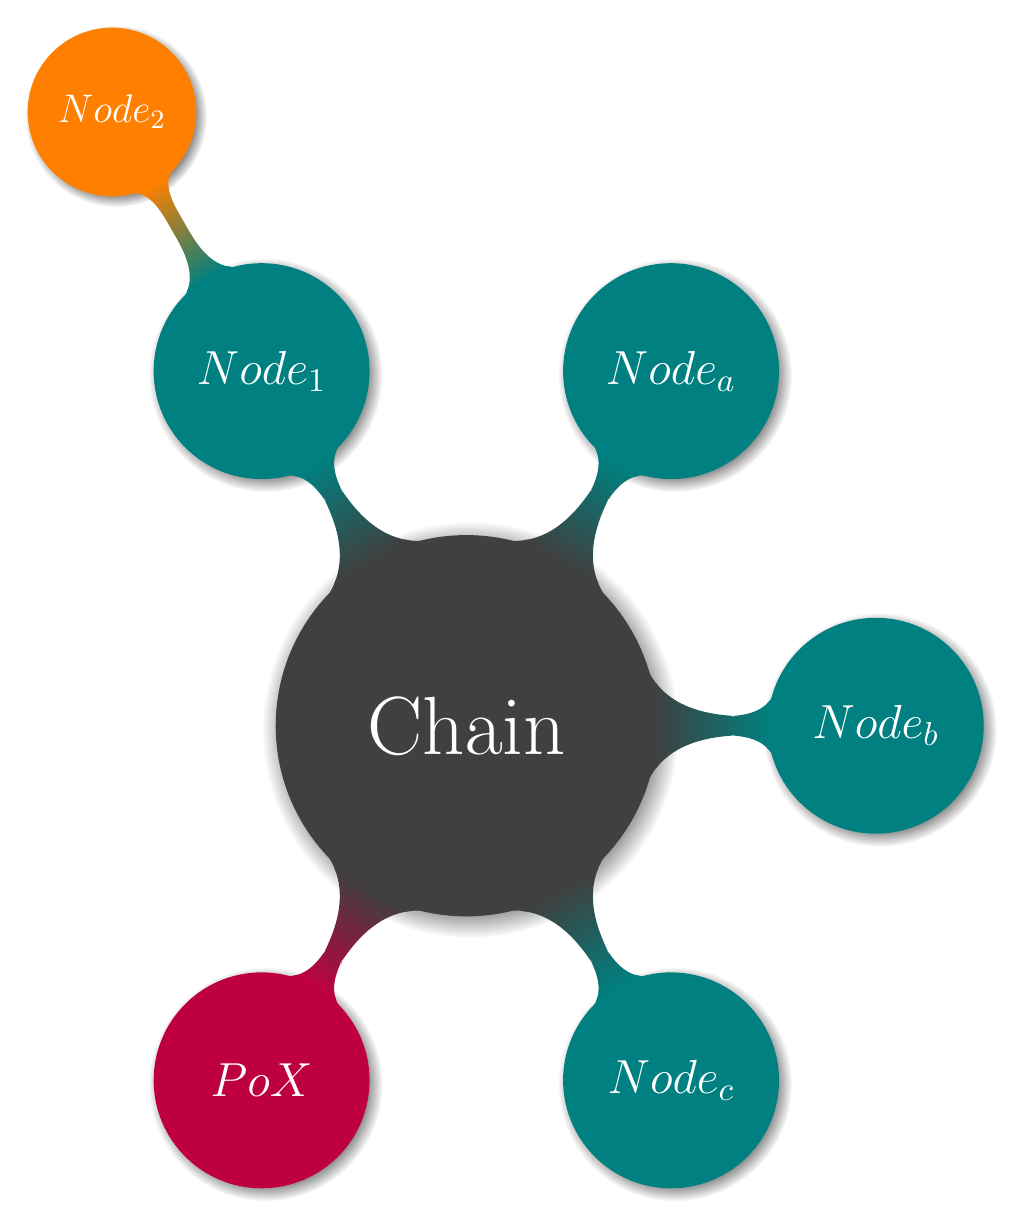
\begin{tikzpicture}
    \path[group]
    node[root] {Chain}
    child[cons] {node {$PoX$}}
    child[node] {node {$Node_c$}}
    child[node] {node {$Node_b$}}
    child[node] {node {$Node_a$}}
    child[node] {node {$Node_1$} child[node,concept color=orange] {node {$Node_2$}}};
  \end{tikzpicture}
  \newpage

  \begin{tikzpicture}
    \path
    node[scale=2,fill=black!15,rounded corners=4mm] (cate) {
    \begin{tikzcd}[catethe,matrix scale=1.4]
      Node_2 \ar[rd, teal, "h"] & Node_1 \ar[d, teal, "g"] \\
      PoX & Chain \ar[l, red] & Node_a \ar[l, teal] \\
      & Node_c \ar[u, teal] & Node_b \ar[lu, teal]
    \end{tikzcd}};
    \anno{$\mathrm{Node_2}$ 首先需要完成惯例的安全检查,之后未同步的数据会从多个节点分块获取,且无需经由 $\mathrm{Node_1}$ 进行中转}{cate.north}{yshift=1cm};
  \end{tikzpicture}
  \qquad\qquad\qquad\qquad\qquad
  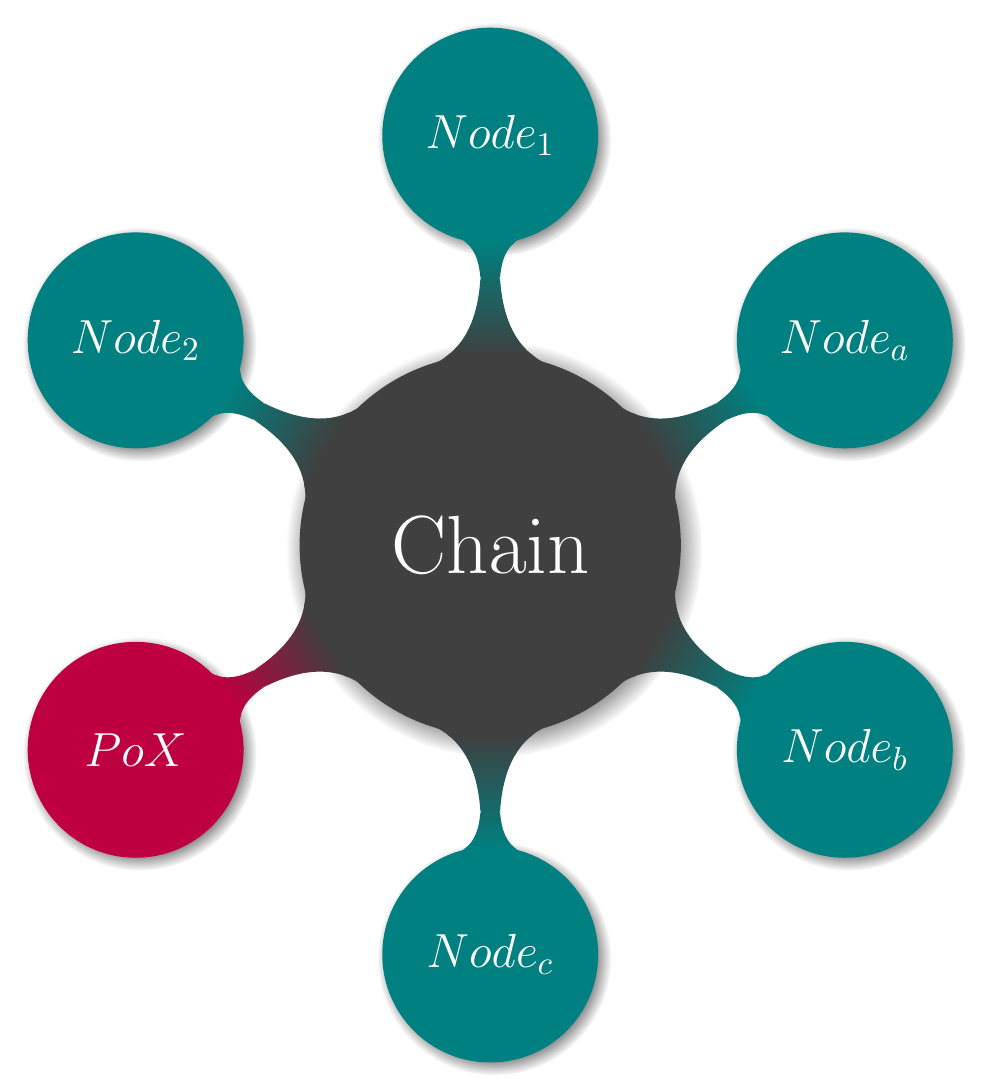
\begin{tikzpicture}
    \path[group]
    node[root] {Chain}
    child[cons] {node {$PoX$}}
    child[node] {node {$Node_c$}}
    child[node] {node {$Node_b$}}
    child[node] {node {$Node_a$}}
    child[node] {node {$Node_1$}}
    child[node] {node {$Node_2$}};
  \end{tikzpicture}

\end{document}
